\documentclass[11pt]{article}

\usepackage[margin=1in]{geometry}
\usepackage{amsmath,amssymb,bm}
\usepackage{booktabs}
\usepackage{graphicx}
\usepackage{hyperref}
\usepackage[numbers]{natbib}

\newcommand{\Rnav}{\mathcal{R}_{\mathrm{nav}}}
\newcommand{\sigmar}{\sigma_r}
\newcommand{\sigmav}{\sigma_v}
\newcommand{\GammaGeom}{\Gamma}
\newcommand{\xstate}{\bm{x}}
\newcommand{\zhat}{\hat{\bm{z}}}
\newcommand{\Phimat}{\bm{\Phi}}
\newcommand{\Qmat}{\bm{Q}}
\newcommand{\Rmat}{\bm{R}}
\newcommand{\Pmat}{\bm{P}}
\newcommand{\Kmat}{\bm{K}}
\newcommand{\Hmat}{\bm{H}}
\newcommand{\Imat}{\bm{I}}


\title{Risk-Aware Adaptive Extended Kalman Filtering for Autonomous Cislunar Spacecraft Navigation}
\author{Fabio Facin}
\date{\today}

\begin{document}
\maketitle

\begin{abstract}
Autonomous spacecraft navigation in cislunar space is an active aerospace
problem because spacecraft cannot always rely on continuous ground support or
Earth-orbit navigation infrastructure. This paper proposes a laptop-scale
computational study of a risk-aware adaptive Extended Kalman Filter (EKF) for
planar Earth-Moon cislunar navigation. The spacecraft dynamics are modeled with
the circular restricted three-body problem (CR3BP), and range-plus-bearing
measurements are simulated under clean and stressed conditions. The proposed
navigation risk score combines covariance growth, measurement geometry,
missed-measurement events, and lighting/visibility penalties. The score adapts
process or measurement noise and is compared with a fixed-noise baseline EKF.
\end{abstract}

\section{Introduction}

Cislunar navigation is becoming increasingly important as lunar and
Earth-Moon-space missions expand. Current research explores autonomous onboard
navigation, optical navigation, cooperative ranging, and robust filtering for
spacecraft operating beyond ordinary GPS coverage
\citep{AerospaceNASA2025Cislunar,NASA2024OpticalNavigation,OguriCislunarAutonomy}.

This project asks a focused computational question: can an interpretable
navigation risk score improve EKF robustness during missed measurements, poor
measurement geometry, and lighting or visibility degradation?

\section{CR3BP Dynamics}

The planar CR3BP state is
\begin{equation}
  \xstate = [x, y, \dot{x}, \dot{y}]^T.
\end{equation}
Using the Earth-Moon mass parameter $\mu$, the nondimensional rotating-frame
equations are
\begin{align}
  \ddot{x} &= 2\dot{y} + x
  - \frac{(1-\mu)(x+\mu)}{r_1^3}
  - \frac{\mu(x-1+\mu)}{r_2^3},\\
  \ddot{y} &= -2\dot{x} + y
  - \frac{(1-\mu)y}{r_1^3}
  - \frac{\mu y}{r_2^3},
\end{align}
where
\begin{equation}
  r_1 = \sqrt{(x+\mu)^2+y^2},\qquad
  r_2 = \sqrt{(x-1+\mu)^2+y^2}.
\end{equation}
The simulator propagates truth and EKF predictions with fourth-order
Runge-Kutta integration.

\section{Measurement Model}

The first measurement model uses range and bearing from a reference observer:
\begin{equation}
  \bm{z} =
  \begin{bmatrix}
  \rho\\
  \theta
  \end{bmatrix}
  =
  \begin{bmatrix}
  \sqrt{(x-x_o)^2+(y-y_o)^2}\\
  \tan^{-1}\left((y-y_o)/(x-x_o)\right)
  \end{bmatrix}
  + \bm{\eta}.
\end{equation}
The measurement Jacobian is analytic and the measurement noise covariance is
$\Rmat$.

\section{Baseline EKF}

The EKF prediction is
\begin{align}
  \hat{\xstate}_{k|k-1} &= f(\hat{\xstate}_{k-1|k-1}),\\
  \Pmat_{k|k-1} &= \Phimat_k \Pmat_{k-1|k-1}\Phimat_k^T + \Qmat.
\end{align}
The measurement update is
\begin{align}
  \Kmat_k &= \Pmat_{k|k-1}\Hmat_k^T
  (\Hmat_k\Pmat_{k|k-1}\Hmat_k^T+\Rmat)^{-1},\\
  \hat{\xstate}_{k|k} &= \hat{\xstate}_{k|k-1}
  + \Kmat_k(\bm{z}_k-\zhat_k),\\
  \Pmat_{k|k} &= (\Imat-\Kmat_k\Hmat_k)\Pmat_{k|k-1}
  (\Imat-\Kmat_k\Hmat_k)^T + \Kmat_k\Rmat\Kmat_k^T.
\end{align}

\section{Navigation Risk Score}

The proposed risk score is
\begin{equation}
\boxed{
\Rnav(t)
=
w_r \frac{\sigmar(t)}{r_0}
+
w_v \frac{\sigmav(t)}{v_0}
+
w_g \frac{1}{\GammaGeom(t)+\epsilon}
+
w_m M(t)
+
w_l L(t)
}
\end{equation}
where $\sigmar=\sqrt{\mathrm{tr}(\Pmat_{rr})}$,
$\sigmav=\sqrt{\mathrm{tr}(\Pmat_{vv})}$, $\GammaGeom$ is a measurement
geometry strength score, $M$ is a missed-measurement flag, and $L$ is a
lighting/visibility penalty.

\section{Adaptive EKF Rules}

The risk score is used in two adaptive filters:
\begin{align}
  \Rmat(t) &= \Rmat_0\left[1+\beta\,\mathrm{clip}(\Rnav,0,R_{\max})\right],\\
  \Qmat(t) &= \Qmat_0\left[1+\alpha\,\mathrm{clip}(\Rnav,0,R_{\max})\right].
\end{align}
The clipping prevents unbounded noise inflation.

\section{Experiments}

The planned experiments compare a baseline EKF, a risk-adaptive measurement
EKF, and a risk-adaptive process EKF across clean and stressed cases:
missed measurements, bad geometry, lighting loss, and combined stress. The
main diagnostics are RMS position error, maximum position error, final velocity
error, covariance growth, maximum risk score, and missed-measurement fraction.

\section{Preliminary Results}

The first controlled scenario suite separated clean navigation, missed
measurements, bad geometry, lighting degradation, and a combined-stress case.
Table~\ref{tab:scenario-summary} summarizes the best filter in each case. The
results show that risk adaptation is not universally beneficial. It is most
useful when the estimator is actually stressed by measurement loss or geometry,
while the fixed baseline remains competitive in clean and lighting-only cases.

\begin{table}[ht]
  \centering
  \caption{First-pass controlled scenario results. RMS errors are nondimensional
  CR3BP position errors from deterministic single-seed runs.}
  \label{tab:scenario-summary}
  \begin{tabular}{lrrrr}
    \toprule
    Scenario & Best filter & Baseline RMS & Best RMS & Improvement\\
    \midrule
    Clean baseline & Baseline & $4.232{\times}10^{-4}$ & $4.232{\times}10^{-4}$ & $0.0\%$\\
    Missed measurements & Adaptive $\Rmat$ & $2.470{\times}10^{-1}$ & $3.632{\times}10^{-3}$ & $98.5\%$\\
    Bad geometry & Adaptive $\Rmat$ & $4.221{\times}10^{-4}$ & $3.075{\times}10^{-4}$ & $27.2\%$\\
    Lighting loss & Baseline & $5.636{\times}10^{-4}$ & $5.636{\times}10^{-4}$ & $0.0\%$\\
    Combined stress & Adaptive $\Qmat$ & $1.005{\times}10^{-3}$ & $8.504{\times}10^{-4}$ & $15.4\%$\\
    \bottomrule
  \end{tabular}
\end{table}

\begin{figure}[ht]
  \centering
  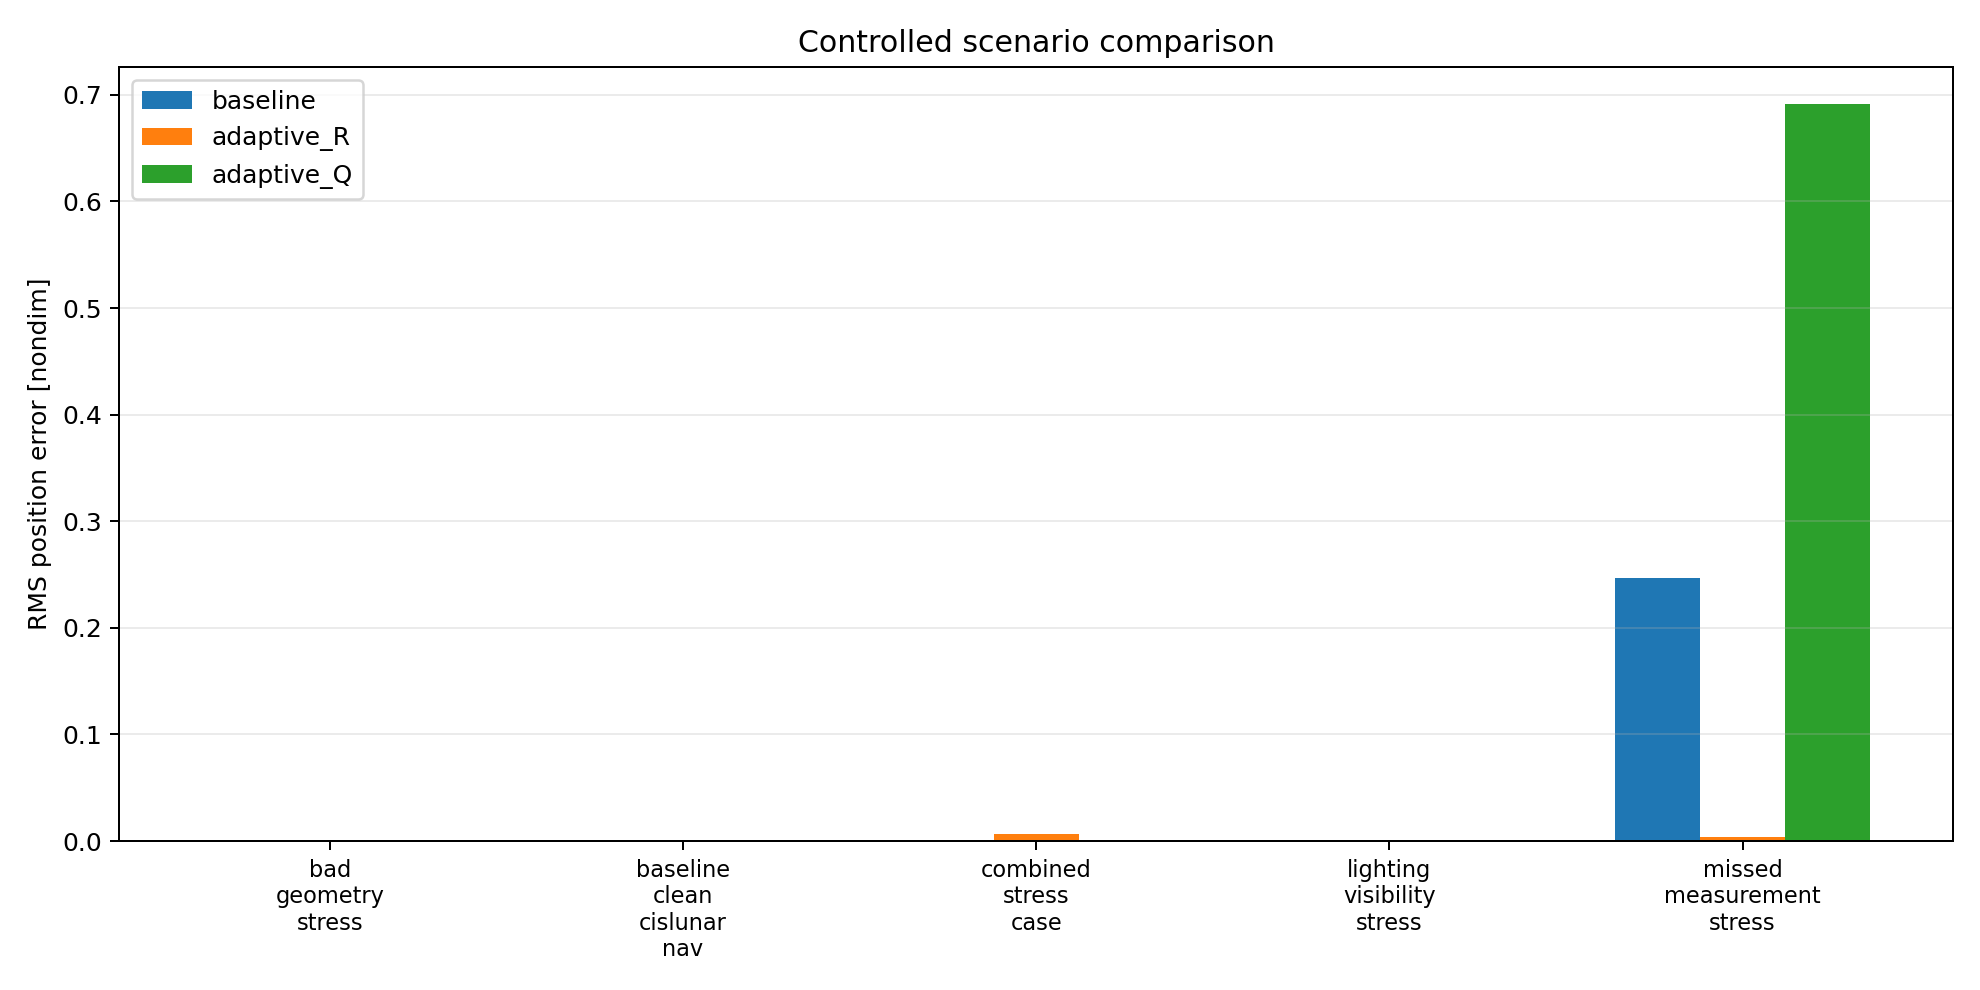
\includegraphics[width=\linewidth]{figures/scenario_rms_comparison.png}
  \caption{RMS position-error comparison across controlled scenarios. The
  adaptive filters help in some stress cases, but the baseline remains best or
  tied in clean and lighting-only cases.}
  \label{fig:scenario-comparison}
\end{figure}

The first implemented parameter scan used a combined-stress scenario with
missed measurements, lighting degradation, and weak geometry. The scan varied
$\alpha$, $\beta$, and $w_g$ over 81 filter summaries. These results are
preliminary; their purpose is to test whether the simulation and comparison
pipeline can expose useful estimator behavior.

The fixed-noise baseline EKF produced an RMS position error of approximately
$1.24$ nondimensional distance units in the combined-stress scan. The best
adaptive measurement-noise case used $\beta=0.6$ and $w_g=0.5$, reducing RMS
position error to approximately $0.589$, a $52.5\%$ improvement over the
same-run baseline. However, more aggressive settings were not uniformly
beneficial. For example, $\beta=1.0$ with $w_g=0.3$ increased RMS position
error to approximately $1.48$ and raised maximum position error to
approximately $9.42$. This confirms that risk-aware adaptation requires
parameter discipline; it is not automatically superior to a standard EKF.

\begin{figure}[ht]
  \centering
  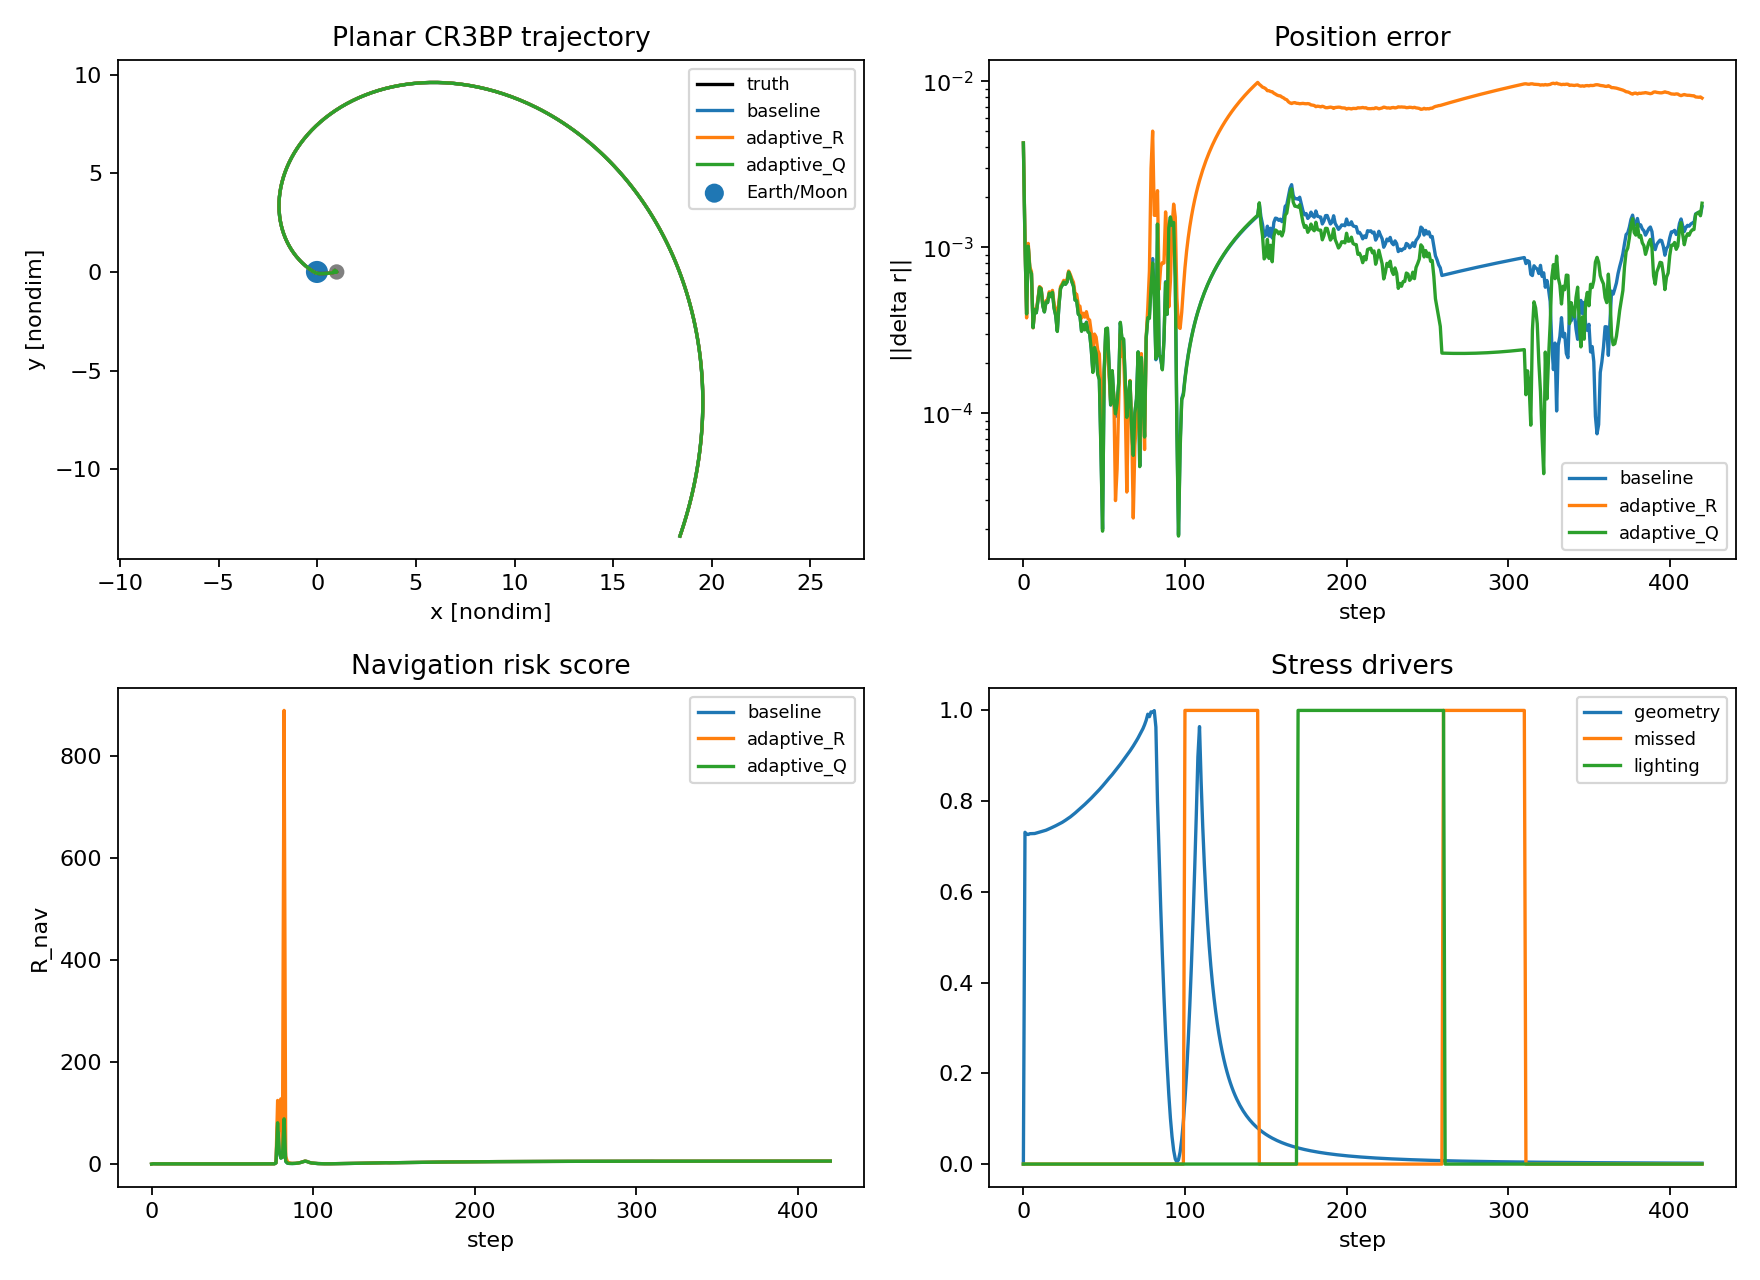
\includegraphics[width=\linewidth]{figures/combined_stress_diagnostics.png}
  \caption{Combined-stress run showing trajectory, position error, navigation
  risk, and stress-driver histories.}
  \label{fig:combined-stress}
\end{figure}

\begin{figure}[ht]
  \centering
  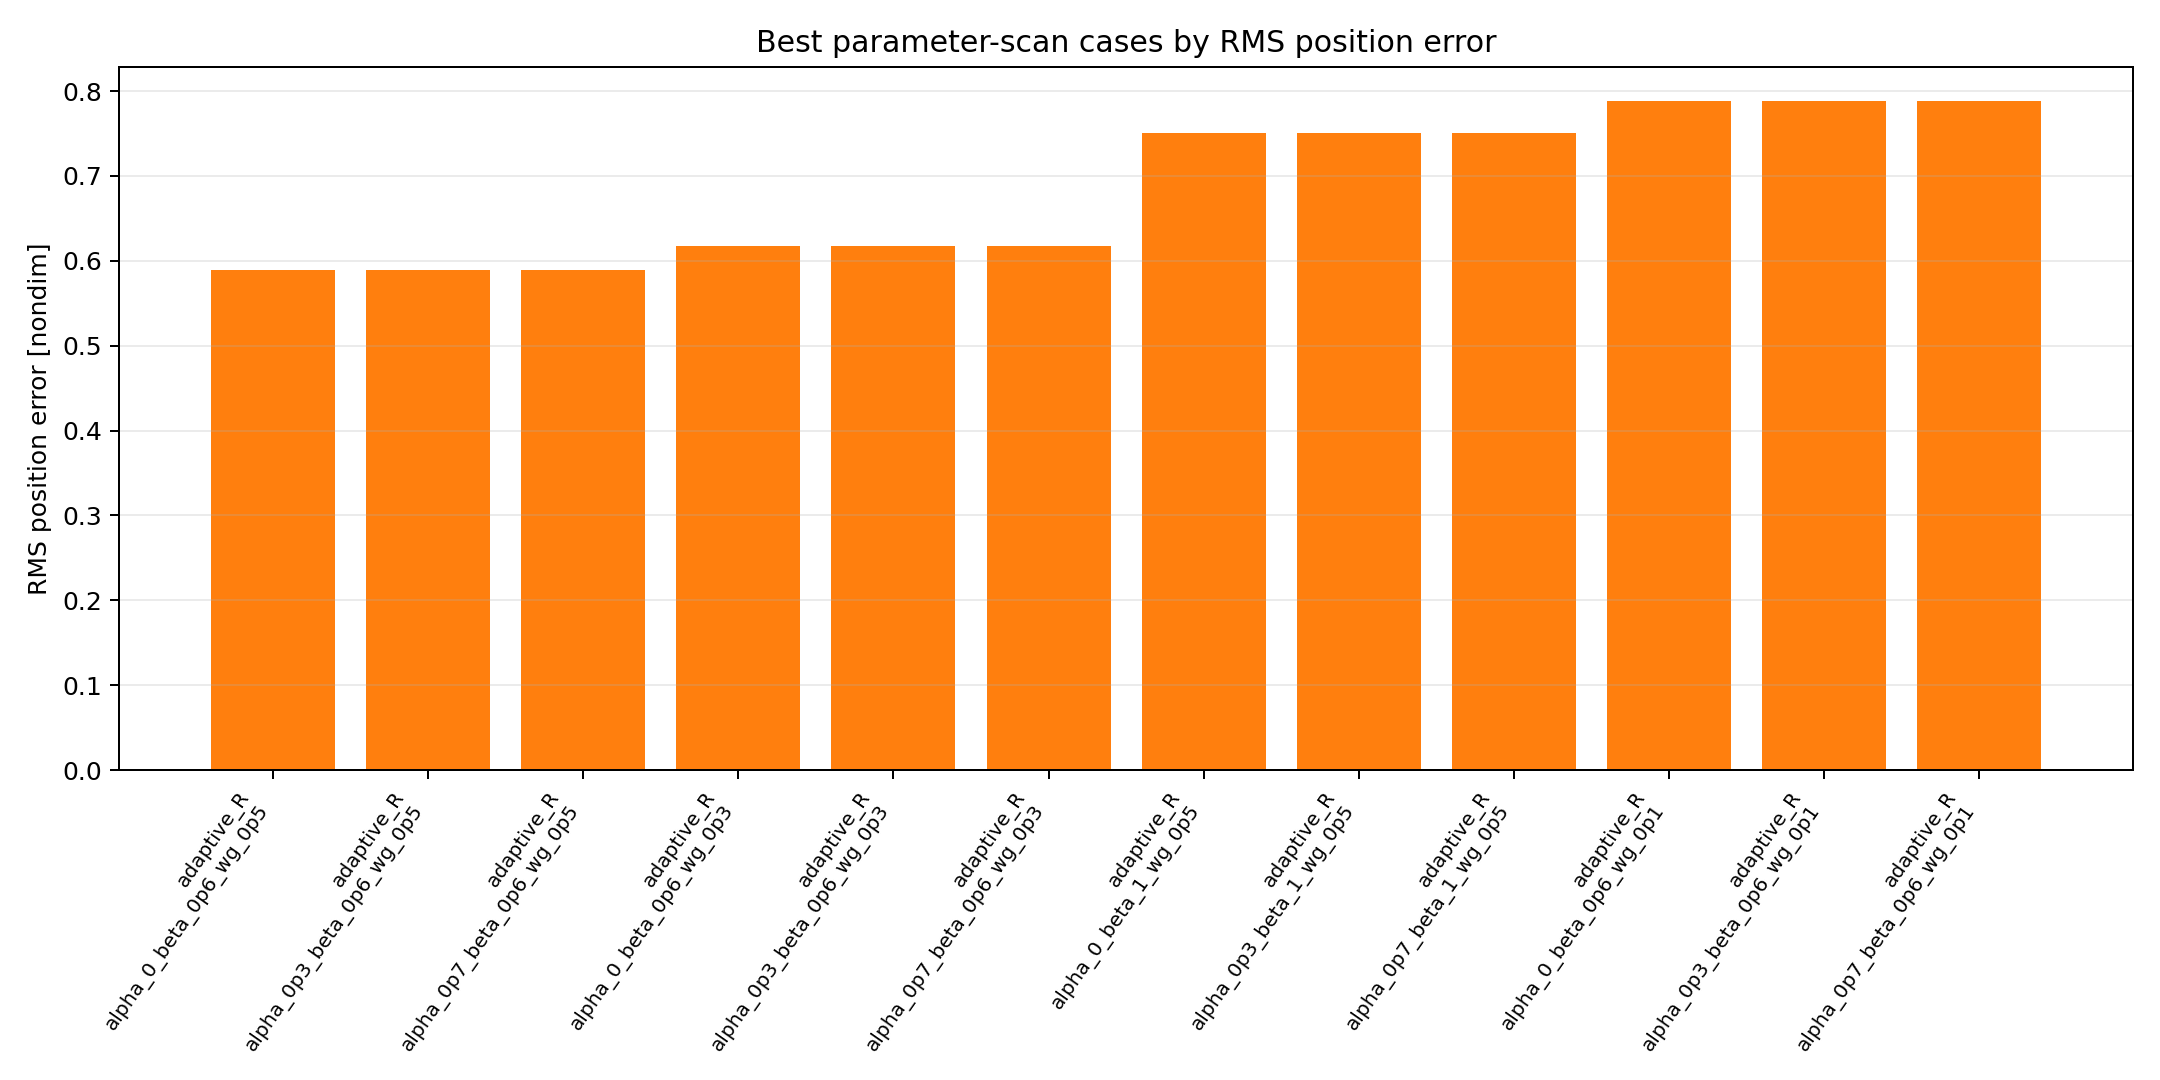
\includegraphics[width=\linewidth]{figures/best_filters.png}
  \caption{Best parameter-scan cases ranked by RMS position error. The best
  early cases use adaptive measurement-noise inflation rather than the fixed
  baseline.}
  \label{fig:best-filters}
\end{figure}

\begin{figure}[ht]
  \centering
  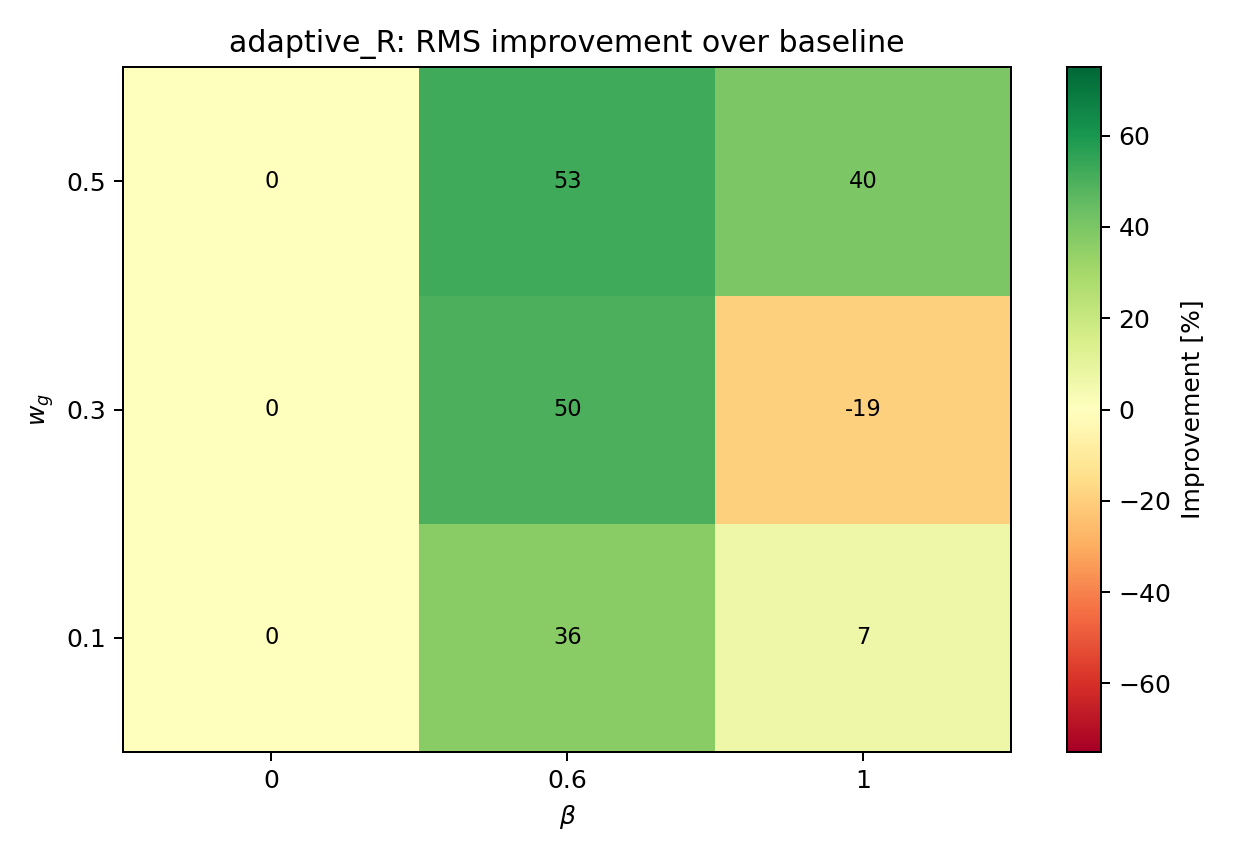
\includegraphics[width=0.78\linewidth]{figures/adaptive_R_improvement_heatmap.png}
  \caption{Adaptive measurement-noise RMS improvement relative to the baseline
  EKF. Green cells indicate improvement; red cells indicate degradation.}
  \label{fig:adaptive-r-heatmap}
\end{figure}

The raw risk score can become very large when the geometry-strength term
$\GammaGeom$ approaches a weak-information regime. This is expected from the
reciprocal form $1/(\GammaGeom+\epsilon)$, but it also means that raw risk
values should be interpreted as diagnostic signals, not direct noise multipliers.
The implemented filters use $\mathrm{clip}(\Rnav,0,R_{\max})$ before adapting
$\Qmat$ or $\Rmat$. The next research step is therefore not simply to maximize
risk response, but to study clipped risk, geometry normalization, and
failure-mode-specific tuning.

\section{Limitations}

This is a v1 computational model. It uses planar CR3BP rather than full
ephemeris dynamics, simplified observers, and simplified visibility penalties.
The purpose is to test estimator behavior under controlled assumptions, not to
claim flight-ready navigation performance. The current result also shows that
the risk equation can be over-sensitive to weak geometry unless its scale and
clipping are treated carefully. This sensitivity is not a reason to discard the
approach; it is a core research target for the next experiments.

\section{Conclusion}

Risk-aware adaptive filtering is a defensible aerospace research direction
because it connects estimator uncertainty to operational stressors. The value
of this project depends on reproducible tests showing when the risk score helps,
when it fails, and whether it improves robustness over a fixed-noise EKF.

\bibliographystyle{plainnat}
\bibliography{references}

\end{document}
